% Geometric multiplicity in 2D: same eigenvalue lambda = 2 (m_a = 2), different eigenspaces.
% Left: 2I, every vector is an eigenvector, E_2 is the whole plane (m_g = 2).
% Right: J_2(2) = [2 1; 0 2], only the x1 axis survives (m_g = 1).
% Same three inputs in both panels: (1,0), (0,1), (-1,1).
\begin{center}
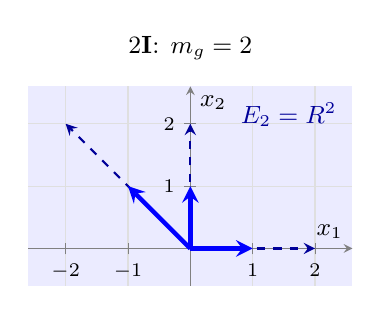
\begin{tikzpicture}
\begin{axis}[
  width=0.47\linewidth,
  axis equal image,
  axis lines=center,
  axis line style={gray},
  xlabel={$x_1$}, ylabel={$x_2$},
  label style={font=\small},
  xmin=-2.6, xmax=2.6, ymin=-0.6, ymax=2.6,
  xtick={-2,-1,1,2}, ytick={1,2},
  tick label style={font=\scriptsize},
  grid=major, grid style={gray!25},
  title={$2\mathbf{I}$: $m_g = 2$}, title style={font=\small},
  % E_2 is the whole plane
  axis background/.style={fill=blue!8},
]
\node[blue!60!black, font=\small, anchor=north east] at (axis cs:2.5,2.5) {$E_2 = \mathbb{R}^2$};
% images, dashed: each lands on its own line
\draw[thick, blue!60!black, -stealth, dashed] (axis cs:0,0) -- (axis cs:2,0);
\draw[thick, blue!60!black, -stealth, dashed] (axis cs:0,0) -- (axis cs:0,2);
\draw[thick, blue!60!black, -stealth, dashed] (axis cs:0,0) -- (axis cs:-2,2);
% inputs, on top
\draw[ultra thick, blue, -stealth] (axis cs:0,0) -- (axis cs:1,0);
\draw[ultra thick, blue, -stealth] (axis cs:0,0) -- (axis cs:0,1);
\draw[ultra thick, blue, -stealth] (axis cs:0,0) -- (axis cs:-1,1);
\end{axis}
\end{tikzpicture}
\hfill
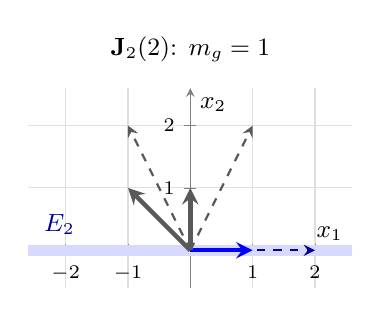
\begin{tikzpicture}
\begin{axis}[
  width=0.47\linewidth,
  axis equal image,
  axis lines=center,
  axis line style={gray},
  xlabel={$x_1$}, ylabel={$x_2$},
  label style={font=\small},
  xmin=-2.6, xmax=2.6, ymin=-0.6, ymax=2.6,
  xtick={-2,-1,1,2}, ytick={1,2},
  tick label style={font=\scriptsize},
  grid=major, grid style={gray!25},
  title={$\mathbf{J}_2(2)$: $m_g = 1$}, title style={font=\small},
]
% E_2 is only the x1 axis
\addplot[domain=-2.6:2.6, line width=4pt, blue!15, samples=2] {0};
\node[blue!60!black, font=\small, anchor=south west] at (axis cs:-2.5,0.1) {$E_2$};
% A e1 = 2 e1 stays on the axis
\draw[thick, blue!60!black, -stealth, dashed] (axis cs:0,0) -- (axis cs:2,0);
% the others are pushed along x1 by the superdiagonal 1: (0,1) -> (1,2), (-1,1) -> (-1,2)
\draw[thick, gray!70!black, -stealth, dashed] (axis cs:0,0) -- (axis cs:1,2);
\draw[thick, gray!70!black, -stealth, dashed] (axis cs:0,0) -- (axis cs:-1,2);
% inputs, on top
\draw[ultra thick, blue, -stealth] (axis cs:0,0) -- (axis cs:1,0);
\draw[ultra thick, gray!70!black, -stealth] (axis cs:0,0) -- (axis cs:0,1);
\draw[ultra thick, gray!70!black, -stealth] (axis cs:0,0) -- (axis cs:-1,1);
\end{axis}
\end{tikzpicture}
\end{center}
